\documentclass[11pt]{article}

\usepackage[a4paper,margin=1in]{geometry}
\usepackage[utf8]{inputenc}
\usepackage[T1]{fontenc}
\usepackage[none]{hyphenat}
\usepackage{amsmath}
\usepackage{amssymb}
\usepackage{graphicx}
\usepackage{booktabs}
\usepackage{caption}
\usepackage{natbib}
\usepackage[hidelinks]{hyperref} 

\sloppy

\title{InkCloser: Line-Art Completion for Paint-Bucket Colorization}

\author{Ruben Tous \\ Computer Architecture Department \\ Universitat Polit\`ecnica de Catalunya \\ Barcelona, Spain \\ \texttt{ruben.tous@upc.edu}}
\date{}

\begin{document}  

\maketitle

\begin{abstract}
Flood-fill (paint-bucket) coloring of line art requires the line drawing to form closed
regions. In practice, line art produced by drawing, scanning, or automatic line extraction
often contains small gaps, and a single gap lets the fill leak across the intended
boundary. We address the problem of restoring such gaps so that a
standard flood-fill tool can be applied without manual retouching. Unlike conventional
image inpainting, the location of the missing content is not available at inference
time. We present InkCloser, a U-Net with gated convolutions, a dilated
context stack, and transformer self-attention at two resolutions. We train it on pairs
built by synthetically removing segments of ink from a collection of clean, closed line-art
images, with a loss that combines pixel-wise cross-entropy, a global Dice term, and
a Dice term restricted to the neighborhood of the removed segments.
We also introduce evaluation metrics that measure gap closing and paint-bucket
behavior directly, rather than relying on pixel accuracy. On a held-out test set, the model closes 70.5\% of the gaps, raises the fraction of
regions that a single bucket click fills correctly (bucket accuracy) from 64.1\% to 94.7\%, reduces
the number of fill leaks per image from 15.5 to 1.5, and makes 45.0\% of the drawings
entirely leak-free. Code, pretrained weights and data are available at \url{https://github.com/rtous/inkcloser}.
\end{abstract}

\section{Introduction}

Two-dimensional cartoon and animation production commonly works with line art: dark strokes on a light background that delimit the regions of a drawing. Such drawings are typically colored with a flood-fill, or paint-bucket, tool, which fills an enclosed region in one click but requires closed contours: where a stroke is interrupted, the fill leaks into the neighboring region. Gaps are common, whether from drawing, scanning, compression, line thinning, or strokes that do not fully close a shape. Most drawing software mitigates this with a gap-closing option that treats openings below a user-set size as closed. This handles many small gaps, but the threshold involves a trade-off: low values let wider gaps leak, while high values also close narrow passages between nearby strokes. 

Our goal is to repair the line art itself: given a drawing with interrupted strokes, we restore the missing ink so that it supports flood-fill coloring without manual correction or per-drawing tuning. This complements the gap-closing options of fill tools, handling gaps beyond their reach and producing line art that is closed for any tool or later pipeline step.

\begin{figure}[t]
  \centering
  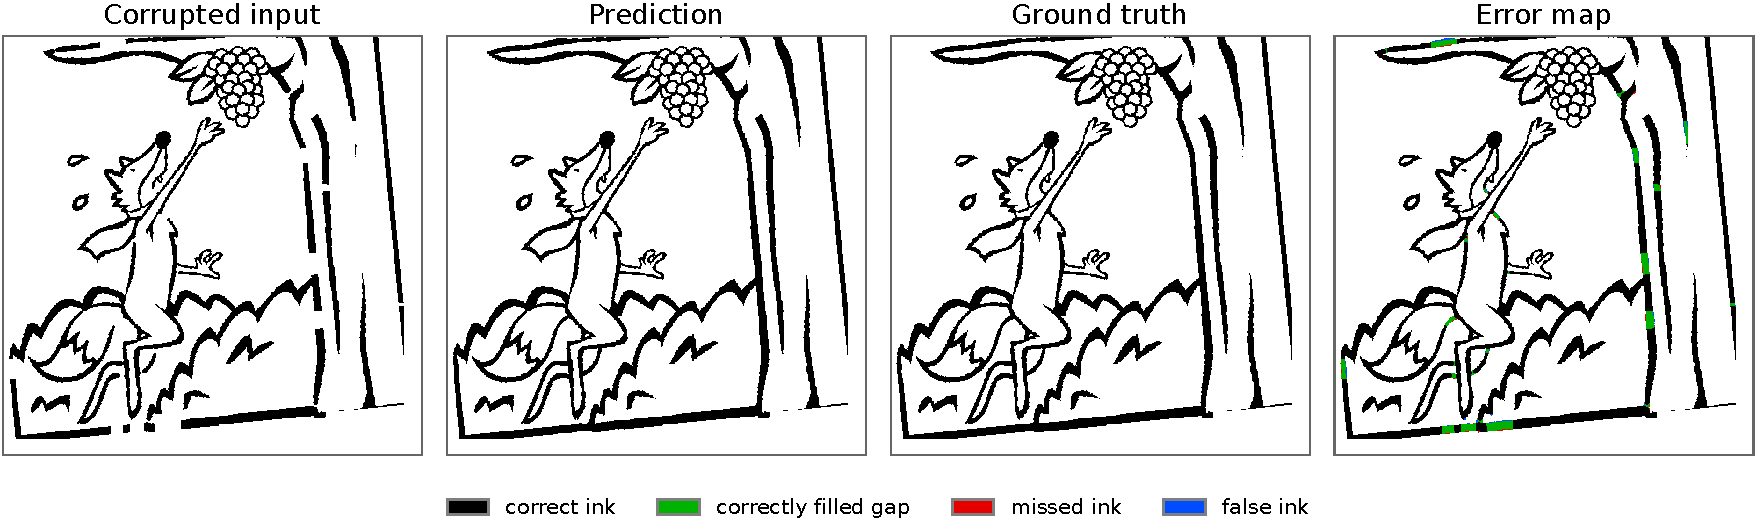
\includegraphics[width=0.9\textwidth]{figures/pair_00000_intro.pdf}
  \caption{Line-art restoration example. From left to right: corrupted input with
missing stroke segments, binarized prediction of our model, ground truth, and
error map.}
  \label{fig:intro}
\end{figure}


The problem is similar to image inpainting, with the key difference that the regions to be filled are not known at inference time. The model must implicitly locate the gaps and close them, while leaving the rest of the drawing unchanged, which makes this a blind, or mask-free, restoration task. A particular difficulty is that not every discontinuity in a line drawing is a defect. Line art routinely contains strokes that end freely by design (e.g. interior detail lines such as folds, wrinkles, etc.). Whether an opening is a gap to be closed or an intentional stroke ending cannot be decided from local geometry alone and can only be learned from examples of complete, correctly closed line art. 

To obtain such examples, we collected images from repositories of coloring pages, which are made specifically to be filled region by region. We generated corrupted inputs by synthetically erasing segments of their ink. We use the resulting dataset to train a network that combines local convolutional processing with global attention, so that it can bridge gaps much longer than a local filter's reach. Because the erased strokes are a tiny fraction of the image, we design the loss function so that the training signal concentrates on them. The contributions of this work are: 

\begin{itemize}
\item A network architecture for mask-free gap closing in line art, which
  locates and bridges gaps without a hole mask, with the goal of enabling
  flood-fill coloring.
\item A loss function that combines hole-weighted cross-entropy with global and
  gap-local Dice terms, focusing training on the erased strokes while preserving
  the intact drawing.
\item A set of evaluation metrics tailored to flood-fill coloring rather than to
  pixel-wise reconstruction, measuring gap closure per erased segment and
  simulating the paint-bucket tool through bucket accuracy and fill leaks.
\item A public dataset of 55\,000 corrupted and clean line-art pairs
  \citep{datasetInkCloser}, together with the code for dataset generation, method
  training and evaluation and the pretrained model weights \citep{codeInkCloser}.
\end{itemize}

\section{Related Work}
\label{sec:related}

\paragraph{Image inpainting.}
Restoring missing strokes resembles image inpainting, in which a network fills a
masked region of an image from its surrounding context. Learned inpainting methods
handle irregular holes by conditioning each convolution on which input pixels are
valid \citep{liu2018partialconv,yu2019gatedconv}, and more recent models enlarge
the receptive field to fill large holes, for example with fast Fourier convolutions
\citep{suvorov2022lama}. These methods assume that a mask of the corrupted region
is given, both during training and at test time. Blind inpainting removes this
assumption: VCNet \citep{wang2020vcnet} first predicts which pixels are corrupted
and then inpaints them, but it targets natural images, where corruption appears as
visible foreign patterns. In line art, a gap is simply missing ink and looks like
background. In our setting the mask is used only to build training pairs: at
inference time the network must also find the gaps it fills.

\paragraph{Gap handling at coloring time.}
The gap problem is well known in cartoon coloring, and the classic remedies avoid
leaks without any learning. Morphological closing of the ink mask
\citep{serra1982morphology,soille2003morphological}, a dilation followed by an
erosion, bridges gaps up to the size of the structuring element, but it also fills
narrow background areas and sharp corners. Trapped-ball segmentation
\citep{zhang2009vectorizing} floods the background with a ball that cannot pass
through gaps narrower than its radius, and LazyBrush \citep{sykora2009lazybrush}
formulates scribble-based coloring as an energy minimization that tolerates small
gaps in the line art. \citet{fourey2018flat} detect stroke endpoints from
contour curvature and close gaps with splines and straight segments, subject to
geometric constraints. Their algorithm is the basis of the line-art detection mode
of the bucket fill tool in GIMP. Delaunay Painting \citep{parakkat2022delaunay} builds a
Delaunay triangulation of the contours and propagates user color hints over it,
which makes coloring robust to large gaps. These methods prevent leaks at coloring
time, but they either do not restore the missing strokes or close them with
hand-designed geometric rules and size thresholds. Recent work also addresses the
opposite problem of small regions left \emph{unpainted} after bucket filling:
GapFill \citep{kono2026gapfill} detects such regions and suggests their colors. This
shows that the paint-bucket workflow is still an active research subject, and the
problem it solves is complementary to ours.

\paragraph{Learned line-art restoration and cleanup.}
Learned approaches instead repair the line art itself. The closest to ours is the
work of \citet{sasaki2017joint}, who train a fully convolutional network on
synthetically corrupted line drawings so that it jointly detects and inpaints gaps
without a mask. The same authors later extended the idea to the restoration of deteriorated
historical drawings \citep{sasaki2018restore}. Related cleanup tasks include sketch
simplification \citep{simoserra2016simplify}, which turns rough sketches into clean lines and has been formulated
with explicit attention to region closure \citep{liu2015closure} and learned with
adversarial augmentation \citep{simoserra2018mastering}, and sketch completion on
vector stroke sequences \citep{lin2020sketchbert}. These works aim at the visual
completion or cleanliness of the drawing, whereas our objective is flood-fill
coloring: we evaluate whether regions are correctly closed, and we design the
architecture and the loss around that goal. We compare with
\citet{sasaki2017joint} directly in Section~\ref{sec:results}.

\paragraph{Line art in animation pipelines.} 
Several recent learning-based tools for 2D animation operate on the regions or
strokes of clean line art and therefore depend on it being well formed.
Reference-based colorization methods match the segments enclosed by the lines
across frames \citep{casey2021animation}. \citet{dai2024inclusion} formulate
paint-bucket colorization as an inclusion-matching problem between segments and
introduce the PaintBucket-Character dataset, and extend the approach to coloring
from character design sheets \citep{dai2024designsheets}. Because these methods
assign one color per enclosed region, a single gap merges two regions and propagates
the error to both. Line inbetweening \citep{siyao2023inbetween} and joint stroke
tracing and correspondence \citep{mo2024jostc} likewise build on vertex or stroke
representations of clean line drawings. Diffusion-based colorization
\citep{liu2025manganinja} does not require closed regions, since it generates
pixel colors directly, but it does not produce the flat, region-wise fills of the
paint-bucket workflow. Our method is a preprocessing step for this family of
region-based tools: it supplies the closed contours that they assume.

\paragraph{Topology-aware losses.}
Closing a gap is a topological rather than a pixel-wise property: a few missing
pixels can merge two regions while barely changing overlap-based losses. In the
segmentation of thin structures such as vessels and roads, this has motivated
losses that explicitly preserve connectivity, using persistent homology
\citep{hu2019topology} or a centerline-based Dice term (clDice)
\citep{shit2021cldice}. Our gap Dice term follows a related intuition with a
simpler mechanism: it concentrates the overlap objective on the neighborhood of the
removed segments, where connectivity is decided.

\section{Problem Statement}  
\label{sec:problem}

Let $Y \in \{0,1\}^{H \times W}$ be a clean line-art image ($0$ for ink, $1$ for
background), and let $X \ge Y$ be a corrupted version in which a subset of ink
pixels, the gap or hole region, has been turned into background. Recovering $Y$
amounts to redrawing the ink in the hole region while leaving the rest of $X$ unchanged. During training we use the hole indicator $h_{ij} = \mathbf{1}[X_{ij} > 0.9 \wedge Y_{ij} < 0.5]$, which marks pixels that are ink in the target and background in the input.

Mask-guided inpainting would learn a mapping that receives both $X$ and the hole
region, so that only the content of the holes must be predicted. We instead learn
a mapping $f_\theta$ with $f_\theta(X) \approx Y$, as in \citet{sasaki2017joint}:
the hole region follows from the pair $(X, Y)$ and is used only during training,
so at inference the network must also locate it, which requires distinguishing
interrupted strokes from strokes that end by design.

\section{Dataset}
\label{sec:dataset}

The InkCloser Dataset is built from 10\,000 clean, closed monochrome line-art images
collected from coloring-page datasets such as the Coloring Book Objects Dataset
\citep{chen2019human}. Each image is resized to $896 \times 896$ pixels, and
corrupted versions are generated by synthetically removing segments of ink.
Corruption is applied in two stages, both operating on the skeleton of the strokes.
The first stage targets T-shaped junctions, where one line meets another: it erases
the first few pixels of the arriving line while keeping the other line intact. This
reproduces a common defect of hand-drawn line art, in which a stroke stops just
short of the line it should touch, and is applied to between 50\% and 100\% of the
eligible junctions of each image. The second stage cuts gaps in the middle of
strokes. To keep the drawings recognizable, at most 35\% of any stroke segment and
25\% of any connected shape is removed, and small shapes such as eyes or highlights
are never corrupted.

The base images are split into 9\,000 for training and 1\,000 for testing. Each
training image has 6 corrupted variants (54\,000 pairs), and each test image has a
single fixed corrupted version (1\,000 pairs). The resulting 55\,000 pairs form the
InkCloser Dataset, which we make public for reproducibility
\citep{datasetInkCloser}.

During training, each time an image is drawn, one of its variants is selected at
random, so the network sees different gap patterns for the same clean image without
corrupting images on the fly. The test set uses a single frozen variant per image,
so that test metrics are reproducible and every method compared in
Section~\ref{sec:results} sees exactly the same gaps.

Training pairs are also augmented. Corruption is applied once, when the dataset is generated, and augmentation is applied afterwards to the corrupted and clean images stacked together, so that both undergo the same random horizontal flip ($p=0.5$), vertical flip ($p=0.2$), rotation (up to $10^{\circ}$), and affine translation and scaling ($\pm 5\%$) with bilinear interpolation and remain pixel-aligned; regions introduced by rotation or translation are filled with white.

\section{Method}
\label{sec:method}

\begin{figure}[t]
  \centering
  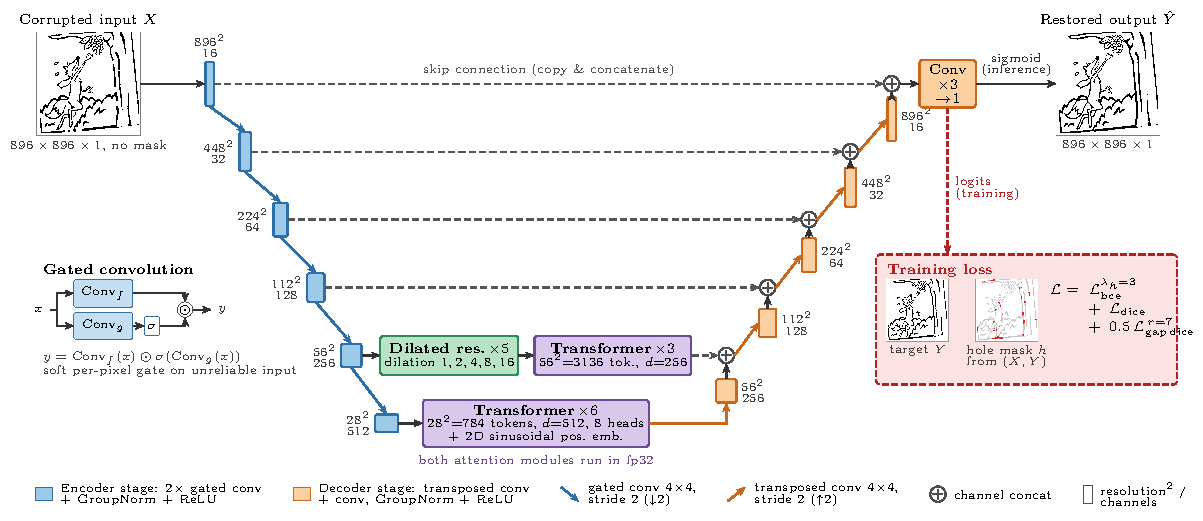
\includegraphics[width=\textwidth]{figures/fig_diagram}
  \caption{Architecture of InkCloser. The corrupted image is processed without a
  hole mask by a U-Net whose encoder uses gated convolutions. Global context is
  added by six transformer blocks at the $28\times 28$ bottleneck and by a dilated
  residual stack followed by three transformer blocks on the $56\times 56$ skip
  connection. The training loss (dashed) uses the target and the hole mask derived
  from the input--target pair. Numbers next to each block give resolution$^2$ and
  channels.}
  \label{fig:overview}
\end{figure}

\subsection{Architecture}
\label{sec:architecture}

The network, illustrated in Figure~\ref{fig:overview}, is an encoder-decoder with
skip connections that operates on single-channel $896\times 896$ images. Every
convolution in the encoder is a gated convolution \citep{yu2019gatedconv}: it
computes a feature map and, in parallel, a sigmoid gate from the same input, and
multiplies the two element-wise. This lets the network learn, at every layer and
spatial location, how much weight to give to each part of the input, which suits
a task in which parts of the input (the gaps) are unreliable by construction.

The encoder has six stages, each consisting of two gated convolutions, each
followed by Group Normalization \citep{wu2018groupnorm} with 8 groups and a ReLU
activation. The first stage operates at full resolution ($896\times 896$) with two
$3\times 3$ convolutions. In each of the following five stages, the first
convolution is $4\times 4$ with stride 2 and halves the spatial resolution, and the
second is $3\times 3$. The resolution thus decreases from $896\times 896$ to
$28\times 28$, while the number of channels doubles from stage to stage (16, 32, 64,
128, 256, 512). 

The decoder mirrors the encoder, following the U-Net skip-connection pattern
\citep{ronneberger2015unet}. Each decoder stage upsamples its input with a
$4\times 4$ transposed convolution of stride 2, followed by a $3\times 3$
convolution, each followed by Group Normalization and a ReLU. The output of each
stage is concatenated with the encoder features of the same resolution before
entering the next stage. The last stage, which returns to $896\times 896$, consists
of the transposed convolution only. After concatenation with the full-resolution
encoder features, a head of three $3\times 3$ convolutions produces a
single-channel logit map at the input resolution.  

Gaps can be long relative to the stroke width and to the receptive field of a stack
of small convolutions. Two modules are therefore added to the U-Net to provide
context across the whole image:
\begin{itemize}
\item \emph{Bottleneck attention.} The $28\times 28$ bottleneck features are
  flattened into a sequence of 784 tokens of dimension 512, a fixed 2D sinusoidal
  positional embedding is added to each token, and the sequence is processed by six
  pre-norm transformer blocks \citep{vaswani2017attention} with 8 attention heads
  and an MLP expansion ratio of 4, followed by a final Layer Normalization. Every
  position can thus attend to every other position, so information about how a
  line continues can be propagated across a gap of any length.
\item \emph{Mid-level context on the skip connection.} The $56\times 56$ encoder
  features (256 channels) are processed before being passed through the skip
  connection to the decoder. They first go through a stack of five residual blocks
  whose first $3\times 3$ convolution has dilation rate 1, 2, 4, 8, and 16,
  respectively, which enlarges the receptive field at low cost. They are then
  processed by three transformer blocks of the same design as above, operating on
  $56\times 56 = 3\,136$ tokens of dimension 256. This gives the decoder access to
  global context at a finer resolution than the bottleneck.
\end{itemize}
Both attention modules are computed in single precision regardless of the mixed
precision setting used elsewhere in the network, which we found necessary for
numerically stable training.

The network outputs logits during training, so that the loss can use a numerically
stable binary cross-entropy formulation. At inference, a sigmoid turns the logits
into a per-pixel probability of background, which is thresholded at 0.5 to obtain
the restored line art. The full model has 43.4\,M parameters.

\subsection{Loss function}

Two properties of the task motivate the design of the loss. First, ink pixels are a
small minority of all pixels, so an unweighted pixel-wise loss is dominated by the
background and gives a weak training signal for the gap-closing behavior we care
about. Second, we want the loss to specifically reward closing the gaps, not only
to reward reproducing the overall image, since a network that copies the input
unchanged already achieves a low loss almost everywhere except at the gaps.

Let $Z$ denote the logit map produced by the network and $p_{ij} = \sigma(Z_{ij})$ the predicted probability of background at pixel $(i,j)$, and let $h_{ij} \in \{0,1\}$ denote the hole indicator defined in Section~\ref{sec:problem}. The loss combines three terms.

\paragraph{Hole-weighted cross-entropy.} A pixel-wise binary cross-entropy term is
computed against the clean target and reweighted so that hole pixels count more
than non-hole pixels:
\begin{equation}
  L_{\mathrm{bce}} = \frac{1}{HW} \sum_{i,j} \bigl(1 + h_{ij}(\lambda_h - 1)\bigr)
  \,\mathrm{BCE}\bigl(Z_{ij}, Y_{ij}\bigr),
\end{equation}
with hole weight $\lambda_h = 3$.

\paragraph{Global Dice.} A Dice loss \citep{milletari2016vnet} is computed between
the predicted ink probability map, $1 - p_{ij}$, and the binarized ink target over
the whole image, which further counters the class imbalance between ink and
background:
\begin{equation}
  L_{\mathrm{dice}} = 1 - \frac{2 \sum_{i,j} (1-p_{ij})\, \mathbf{1}[Y_{ij}<0.5] + \epsilon}
  {\sum_{i,j} (1-p_{ij}) + \sum_{i,j} \mathbf{1}[Y_{ij}<0.5] + \epsilon}.
\end{equation}

\paragraph{Gap Dice.} The same Dice term is computed a second time, restricted to a
neighborhood of the hole region obtained by dilating the hole mask with a
$(2r+1)\times(2r+1)$ max-pooling window, $r=7$ pixels. This term is zero for images
without gaps and otherwise focuses the Dice objective specifically on the completed
regions, independently of how well the rest of the image is reconstructed.

The total loss is
\begin{equation}
  L = \beta_{\mathrm{bce}} L_{\mathrm{bce}} + \beta_{\mathrm{dice}} L_{\mathrm{dice}}
  + \beta_{\mathrm{gap}} L_{\mathrm{gap\,dice}},
\end{equation}
with $\beta_{\mathrm{bce}} = 1.0$, $\beta_{\mathrm{dice}} = 1.0$, and
$\beta_{\mathrm{gap}} = 0.5$. In preliminary experiments, a much larger hole weight
($\lambda_h = 8$) caused the network to over-predict ink outside the hole regions;
the milder weight of 3, combined with the Dice terms, gave a better balance between
filling gaps and preserving the rest of the drawing.

\subsection{Training procedure}

The network is trained with AdamW \citep{loshchilov2019adamw} and weight decay
$10^{-4}$, using two learning rates: $10^{-3}$ for all convolutional parameters and
$3\times 10^{-4}$ for the parameters of the two attention modules. The learning
rate is decayed with a cosine annealing schedule \citep{loshchilov2017sgdr}. Training uses mixed-precision forward and backward passes
with gradient scaling, and gradients are clipped to a maximum norm of 1.0. The batch
size is 4, giving 2\,250 optimization steps per pass over the 9\,000 training images.
The reported model was trained for 5 epochs.

\section{Evaluation Protocol and Metrics}
\label{sec:metrics}

Pixel-wise accuracy or a plain pixel F1 score is a poor proxy for the quality of the
restoration in this task, for two reasons: ink pixels are a small fraction of the
image, so a model that never adds any ink already scores well on pixel accuracy;
and pixel overlap does not directly say whether the regions that flood fill depends
on were actually recovered. We therefore report metrics at three levels: the ink
added by a method, the individual erased segments, and the background regions that a
paint-bucket tool would fill. Global pixel metrics are reported for reference.

All metrics are computed on the binarized output. A pixel is ink if its value is
below 0.5 on a $[0,1]$ scale, and the network's probability map is thresholded at
0.5. A region is a 4-connected component of background pixels, which pairs correctly
with 8-connected ink strokes; background components smaller than 20 pixels are
ignored, since they are specks rather than paintable regions. Unless
noted otherwise, metrics are pooled over the whole test set (micro-averaged). Counts
are summed over all images and the ratio is taken once.

\paragraph{Fill precision, recall, and F1.} These metrics consider only the ink that
a method adds. Let $\text{added}$ be the set of pixels that are ink in the output but
background in the corrupted input, and let $\text{gap}$ be the set of pixels that are
ink in the clean target but background in the corrupted input (the ground-truth hole
region). With a pixel tolerance $\tau$ (a match within $\tau$ pixels, via
morphological dilation, counts as correct), fill precision is the fraction of added
pixels that lie within $\tau$ pixels of the ground-truth ink, and fill recall is the
fraction of gap pixels that lie within $\tau$ pixels of the added ink. Fill F1 is
their harmonic mean. We report $\tau = 0$ (exact) and $\tau = 2$. The exact setting
is strict: a correctly placed stroke that is one pixel thicker than the target is
penalized. The tolerant setting separates errors in line thickness or position from
missing structure.

\paragraph{Pixel metrics.} Pixel IoU and pixel F1 between the output ink and the
ground-truth ink over the whole image; \emph{ink kept}, the fraction of the input's
ink pixels that remain ink in the output, which checks that a method does not erase
existing lines; and the \emph{ink ratio}, the total output ink divided by the total
ground-truth ink, which is 1 in the ideal case, above 1 when lines are too thick or
spurious ink is added, and below 1 when ink is missing.

\paragraph{Gap closure.} An erased segment is an 8-connected component of the
ground-truth hole region, ignoring components of fewer than 4 pixels. A segment is
counted as closed if at least 80\% of its pixels are ink in the output. Gap closure is
the fraction of erased segments that are closed. The length of a segment is the
longer side of its bounding box, in pixels, which we use to analyze performance as a
function of gap size.

\paragraph{Region and paint-bucket metrics.} These metrics measure the practical goal
of the task most directly. \emph{Region count accuracy} is the fraction of images in
which the output has exactly as many regions as the ground truth; it is a strict,
whole-image metric, since a single missed or spurious gap changes the count.
\emph{Region recovery} is the fraction of regions merged by the gaps (ground-truth
region count minus input region count, summed over images) that are separated again
in the output. To simulate the paint-bucket tool, each ground-truth region is matched
to the output region with the highest IoU with it; the region is \emph{correctly
paintable} if that IoU is at least 0.9. \emph{Bucket accuracy} is the fraction of
ground-truth regions that are correctly paintable, which approximates the fraction of
regions that a user could fill correctly with a single click, and \emph{mean region
IoU} is the average best-match IoU over all ground-truth regions. Finally, a
\emph{leak} occurs when one output region contains at least 50\% of each of two or
more ground-truth regions, so that a single bucket fill would spill across them; an
output region that absorbs $k$ ground-truth regions counts as $k-1$ leaks. We report
the mean number of \emph{leaks per image} and the fraction of \emph{leak-free images},
that is, drawings that are fully ready to color without manual correction.

\paragraph{Statistical analysis.} We report 95\% percentile bootstrap confidence
intervals \citep{efron1994bootstrap} computed over test images (1\,000 resamples).
The same resamples are used for all methods, so differences between methods are
paired, and we report one-sided paired bootstrap tests of the proposed method against
each baseline.

\paragraph{Baselines.} As no mask is available at inference time, mask-guided
inpainting methods are not directly applicable. We compare against the following
methods, all of which operate under the same mask-free, single-image setting and are
evaluated on exactly the same test pairs with the same metric code:
\begin{itemize}
\item \emph{Input (no restoration)}: the corrupted image evaluated as if it were the
  output. It serves as a no-op reference and quantifies the damage caused by the gaps. Since it
  adds no ink, fill precision and fill F1 are undefined for it.
\item \emph{Morphological closing} \citep{serra1982morphology,soille2003morphological}
  (Section~\ref{sec:related}), with an elliptical structuring element of diameter
  $k \in \{5, 9\}$ pixels. It is the classical training-free way to close gaps and
  is essentially what the ``close gap'' options of drawing software do.
\item \emph{\citet{sasaki2017joint}}: the joint gap detection and
  inpainting network, a fully convolutional encoder-decoder without skip connections
  (5.5\,M parameters). The official release targets Torch7; we converted the released
  weights layer by layer into an identical PyTorch network and followed the authors'
  pre- and post-processing (normalization with the stored mean and standard deviation,
  white padding to a multiple of 16, and their output sharpening step, which does not
  change which pixels are ink at the 0.5 threshold). We evaluate two variants.
  \emph{Pretrained}: the released weights applied zero-shot, with no training on our
  data. The only adaptation considered was the resolution at which the network runs;
  the scale factor was selected by fill F1 on 64 training images (never on test
  images), and the best choice was the native resolution (scale 1). \emph{Retrained}:
  the same architecture trained from random initialization on our training pairs, with
  the same augmentation as our model, following the original training recipe (mean
  squared error loss and the AdaDelta optimizer \citep{zeiler2012adadelta}) on random
  $448\times 448$ crops, and evaluated on the full test images. The last checkpoint of
  the run is reported, so no model selection was performed on test data. This variant controls for the training data and augmentation.
\end{itemize}

\section{Results}
\label{sec:results}

All results are computed on the full frozen test set of 1\,000 images and 26\,141
erased segments. Every method is evaluated on the same corrupted images and with the
same metric code, and the bootstrap confidence intervals of all methods use the same
resamples. Table~\ref{tab:main_results} reports the main metrics with their
confidence intervals.

\begin{table}[t]
\centering
\caption{Line restoration on the held-out test set (1\,000 images, 26\,141 erased
segments). Values are percentages unless noted; $\pm$ is half the width of the 95\%
bootstrap confidence interval. $\tau$: pixel tolerance. Bucket acc.: ground-truth
regions recovered with IoU$\geq$0.9. Leak: one output region spanning two
ground-truth regions. $\uparrow$: higher is better; $\downarrow$: lower is better;
$\to 1$: closest to 1 is best. Best value per column in bold.}
\label{tab:main_results}
\small
\resizebox{\linewidth}{!}{%
\begin{tabular}{lcccccccccc}
\toprule
 & \multicolumn{4}{c}{Added ink} & \multicolumn{2}{c}{Whole image} & Segments & \multicolumn{3}{c}{Paint bucket} \\
\cmidrule(lr){2-5} \cmidrule(lr){6-7} \cmidrule(lr){8-8} \cmidrule(lr){9-11}
Method & \shortstack{Fill P\\($\tau$=0) $\uparrow$} & \shortstack{Fill R\\($\tau$=0) $\uparrow$} & \shortstack{Fill F1\\($\tau$=0) $\uparrow$} & \shortstack{Fill F1\\($\tau$=2) $\uparrow$} & \shortstack{Pixel\\F1 $\uparrow$} & \shortstack{Ink\\ratio $\to 1$} & \shortstack{Gap\\closure $\uparrow$} & \shortstack{Bucket\\acc. $\uparrow$} & \shortstack{Leaks /\\image $\downarrow$} & \shortstack{Leak-free\\images $\uparrow$} \\
\midrule
Input (no restoration) & -- & 0.0{\scriptsize$\pm$0.0} & -- & -- & 98.4{\scriptsize$\pm$0.0} & 0.968{\scriptsize$\pm$0.001} & 0.0{\scriptsize$\pm$0.0} & 64.1{\scriptsize$\pm$1.6} & 15.46{\scriptsize$\pm$0.66} & 0.1{\scriptsize$\pm$0.1} \\
Closing ($k$=5) & 1.1{\scriptsize$\pm$0.1} & 1.8{\scriptsize$\pm$0.1} & 1.4{\scriptsize$\pm$0.1} & 11.6{\scriptsize$\pm$0.4} & 95.9{\scriptsize$\pm$0.1} & 1.021{\scriptsize$\pm$0.003} & 1.4{\scriptsize$\pm$0.2} & 37.6{\scriptsize$\pm$1.1} & 13.08{\scriptsize$\pm$0.58} & 0.2{\scriptsize$\pm$0.2} \\
Closing ($k$=9) & 1.2{\scriptsize$\pm$0.1} & 6.3{\scriptsize$\pm$0.2} & 2.1{\scriptsize$\pm$0.1} & 25.2{\scriptsize$\pm$0.7} & 91.1{\scriptsize$\pm$0.4} & 1.129{\scriptsize$\pm$0.009} & 6.3{\scriptsize$\pm$0.4} & 22.8{\scriptsize$\pm$1.1} & 9.45{\scriptsize$\pm$0.43} & 0.3{\scriptsize$\pm$0.4} \\
Sasaki et al.\ (pretrained) & 10.7{\scriptsize$\pm$0.5} & 54.0{\scriptsize$\pm$1.0} & 17.8{\scriptsize$\pm$0.7} & 81.9{\scriptsize$\pm$0.6} & 90.1{\scriptsize$\pm$0.3} & 1.081{\scriptsize$\pm$0.003} & 26.6{\scriptsize$\pm$0.8} & 26.2{\scriptsize$\pm$1.5} & 13.77{\scriptsize$\pm$1.38} & 4.2{\scriptsize$\pm$1.2} \\
Sasaki et al.\ (retrained) & 28.1{\scriptsize$\pm$1.3} & 56.5{\scriptsize$\pm$1.3} & 37.6{\scriptsize$\pm$1.4} & 87.2{\scriptsize$\pm$0.7} & 94.1{\scriptsize$\pm$0.2} & 0.974{\scriptsize$\pm$0.001} & 20.8{\scriptsize$\pm$1.1} & 36.4{\scriptsize$\pm$2.1} & 19.36{\scriptsize$\pm$1.87} & 8.5{\scriptsize$\pm$1.6} \\
Ours & \textbf{73.6}{\scriptsize$\pm$1.0} & \textbf{84.0}{\scriptsize$\pm$0.6} & \textbf{78.5}{\scriptsize$\pm$0.7} & \textbf{92.8}{\scriptsize$\pm$0.5} & \textbf{99.3}{\scriptsize$\pm$0.0} & \textbf{1.004}{\scriptsize$\pm$0.000} & \textbf{70.5}{\scriptsize$\pm$0.9} & \textbf{94.7}{\scriptsize$\pm$0.4} & \textbf{1.47}{\scriptsize$\pm$0.14} & \textbf{45.0}{\scriptsize$\pm$3.0} \\
\bottomrule
\end{tabular}}
\end{table}

\paragraph{Paint-bucket behavior.} The metrics that measure the actual goal of the
task show the largest effect. On the unrestored input, only 64.1\% of the
ground-truth regions can be filled correctly with a single bucket click, each image
has on average 15.5 leaks, and only 1 of the 1\,000 images is leak-free. After
restoration with our model, bucket accuracy rises to 94.7\%, the number of leaks per
image drops by 90.5\% to 1.47, and 45.0\% of the drawings (450 images) are entirely
leak-free and ready to color without any manual correction. Most restored images have few leaks: 66.9\% have at most one leak and
78.5\% have at most two, compared with a median of 13 leaks per image on the input.
Of the 15\,458 regions that the gaps merge across the test set, 94.0\% are separated
again, and the mean best-match IoU of the ground-truth regions rises from 70.9\% to
96.5\%. Region count accuracy, the strictest whole-image metric, rises from 0.1\% to
38.0\%. Our model is the only method in Table~\ref{tab:main_results} that improves
on the bucket accuracy of the unrestored input; every other method lowers it.

\paragraph{Comparison with morphological closing.} Morphological closing fails on
this task. With $k = 9$ it closes only 6.3\% of the erased segments and recovers
6.3\% of the missing ink. Although it reduces the number of leaks per image (from
15.5 to 9.4), it does so largely by filling narrow background areas and thickening
junctions, which destroys small regions rather than separating merged ones: its
bucket accuracy drops to 22.8\%, well below that of the unrestored input (64.1\%),
its ink ratio rises to 1.13, and its pixel F1 falls below that of the input. The
smaller kernel ($k = 5$) damages the drawing less but closes almost no gaps (1.4\%).
Both effects are visible in the second column of Figure~\ref{fig:qualitative}, where closing merges nearby strokes into ink blobs
while leaving most gaps open. The fill precision of closing at $\tau = 2$ is high
(100.0\% for $k=5$, 91.3\% for $k=9$) only because a dilation can add ink solely next
to existing strokes; its recall at the same tolerance remains low (6.1\% and 14.6\%).

\paragraph{Comparison with Sasaki et al.} The network of \citet{sasaki2017joint}
performs clearly better than closing at the ink level, but it does not make the
drawings paintable. With its released weights, applied zero-shot, it redraws 54.0\%
of the erased ink and closes 26.6\% of the erased segments, the highest gap closure
among the baselines. However, only 10.7\% of the ink it adds lies exactly on a
ground-truth stroke, its ink ratio is 1.08, and it keeps only 95.1\% of the ink of
the input: the network redraws the whole drawing in the style of its own training
data, with thicker strokes and small spurious marks, rather than only filling the
gaps. As a consequence, it re-separates 60.6\% of the merged regions but correctly
recovers only 26.2\% of the ground-truth regions, and only 4.2\% of the images are
leak-free. This variant was trained on different drawings, with different line widths
and gap statistics, so these numbers measure zero-shot generalization rather than the
capacity of the approach; changing the input scale did not improve its fill F1 on
training images (Section~\ref{sec:metrics}).

Retrained on our training pairs, the same architecture adapts to the line style of
our data: its fill precision rises to 28.1\% (97.6\% at $\tau=2$), its fill F1 to
37.6\%, and its ink ratio (0.974) is close to that of the input. Its gap closure,
however, decreases to 20.8\%, its region recovery to 33.7\%, and the number of leaks
per image increases to 19.4, above that of the unrestored input (15.5). We attribute
this mainly to the fact that the network regenerates every stroke rather than copying
the input where it is intact: it keeps only 94.1\% of the input ink, and its error
maps (Figure~\ref{fig:qualitative}) show missed and false pixels along almost every
existing stroke, not only at the gaps. Thin and faint strokes are partly lost in this
process, which opens new gaps, and therefore new leaks, elsewhere in the drawing. Its
results also vary strongly between images (Figure~\ref{fig:boxplots}): its per-image
bucket accuracy spans the whole range from 0 to 1, with a median of 48.3\%, whereas
ours has a median of 96.4\%. Since this variant uses the same training data,
augmentation, and test protocol as our model, the difference between the two, 49.7
percentage points in gap closure and 58.4 in bucket accuracy, reflects the combined
effect of our architecture and training objective. We attribute this to the skip connections and gated convolutions, which allow intact strokes to pass through unchanged (our model keeps 99.9998\% of the input ink), and to the attention modules and the hole-focused loss, which focus its capacity on the gaps.

\paragraph{Statistical significance.} Our model outperforms the input, both closing
variants, and both Sasaki et al.\ variants on all four key metrics (fill F1, gap
closure, bucket accuracy, and leak-free images), with paired-bootstrap $p \le 0.001$ in
every comparison (Table~\ref{tab:significance}). The per-image distributions in
Figure~\ref{fig:boxplots} confirm that the improvement is not driven by a subset of
easy images: the first quartile of the per-image bucket accuracy of our model
(92.0\%) is higher than the median of every other method, and higher than the upper
whisker of both closing variants.

\begin{table}[t]
\centering
\caption{Paired bootstrap comparison of our model against each baseline: difference
(ours minus baseline, percentage points) with its 95\% confidence interval, computed
with the same 1\,000 resamples of test images for all methods. All differences are
significant with a one-sided $p \le 0.001$ (the smallest attainable value with 1\,000 resamples). Fill F1 is undefined for the input.}
\label{tab:significance}
\small
\setlength{\tabcolsep}{3pt}
\begin{tabular}{lcccc}
\toprule
Baseline & Fill F1 ($\tau$=0) & Gap closure & Bucket acc. & Leak-free images \\
\midrule
Input (no restoration) & -- & +70.5 [69.5, 71.4] & +30.7 [29.3, 32.1] & +44.9 [41.9, 47.9] \\
Closing ($k$=5) & +77.1 [76.4, 77.8] & +69.1 [68.1, 70.0] & +57.2 [56.1, 58.3] & +44.8 [41.7, 47.8] \\
Closing ($k$=9) & +76.4 [75.7, 77.1] & +64.1 [63.1, 65.1] & +72.0 [70.8, 73.1] & +44.7 [41.6, 47.7] \\
Sasaki et al.\ (pretrained) & +60.7 [60.0, 61.3] & +43.9 [43.0, 44.8] & +68.5 [67.0, 70.1] & +40.8 [37.8, 43.7] \\
Sasaki et al.\ (retrained) & +40.9 [39.8, 42.1] & +49.7 [48.7, 50.6] & +58.4 [56.3, 60.5] & +36.5 [33.6, 39.4] \\
\bottomrule
\end{tabular}
\end{table}

\begin{figure}[t]
  \centering
  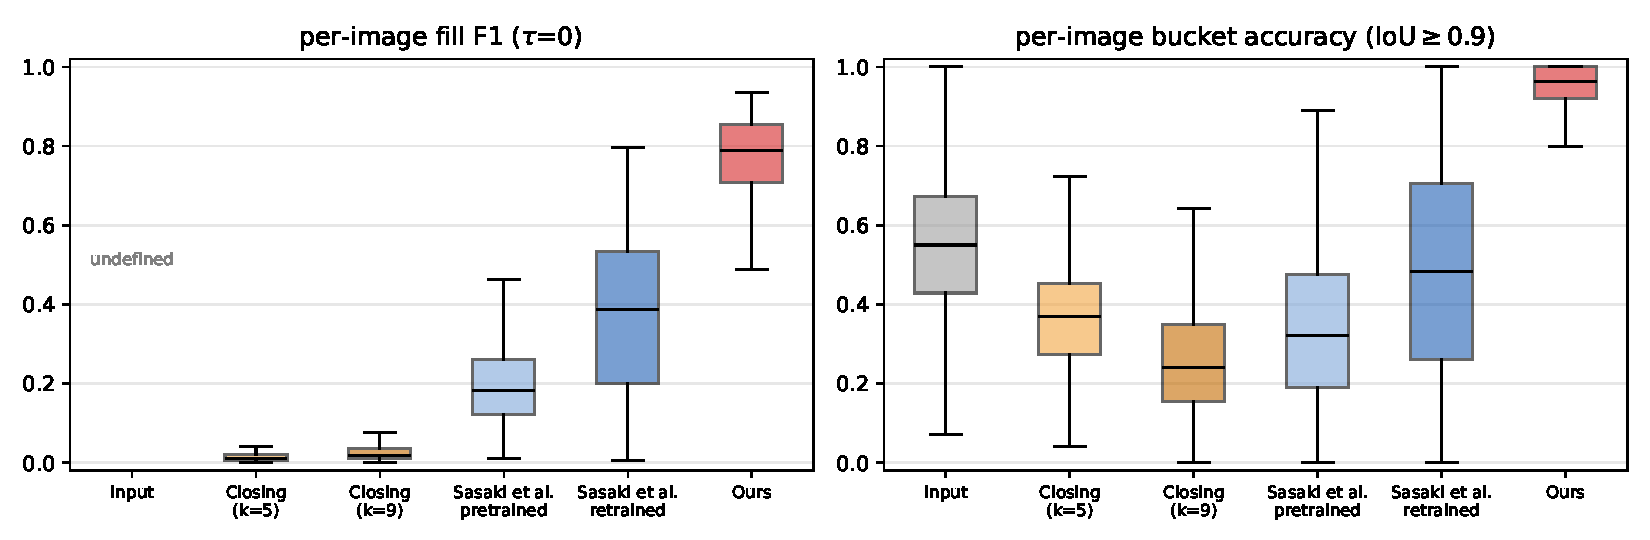
\includegraphics[width=\textwidth]{figures/fig_per_image_boxplots_all.pdf}
  \caption{Per-image distributions over the 1\,000 test images of the fill F1 at
  $\tau=0$ (left) and of the bucket accuracy (right). Boxes show the interquartile
  range and the median; whiskers extend to 1.5 times the interquartile range;
  outliers are hidden. Fill F1 is undefined for the input.}
  \label{fig:boxplots}
\end{figure}

\paragraph{Ink-level accuracy.} Our model recovers 84.0\% of the erased ink exactly
and places 73.6\% of the ink it adds exactly on the ground-truth strokes, for a fill
F1 of 78.5\%. With a tolerance of two pixels, fill precision, recall, and F1 rise to
91.7\%, 93.9\%, and 92.8\%, which indicates that most of the remaining pixel-level
error is a matter of stroke thickness or position along the stroke boundary rather
than missing or hallucinated structure. The model preserves the input:
it keeps 99.9998\% of the ink already present in the corrupted image, and its ink
ratio (1.004) shows that the restored lines are neither systematically thicker nor
thinner than the target. Pixel F1 and pixel IoU are high for all methods, including
the unrestored input (98.4\% pixel F1), because most ink is untouched by the
corruption; they confirm that the model does not degrade the drawing (99.3\% pixel
F1) but are not informative for ranking methods. Every baseline, including both
Sasaki et al.\ variants, has a lower pixel F1 than the unrestored input, because the ink it removes or adds incorrectly outweighs the ink it recovers.

\paragraph{Effect of gap length.} Table~\ref{tab:gap_length} and
Figure~\ref{fig:gap_length} break down gap closure by the length of the erased
segment. Morphological closing only closes gaps that are short relative to its
kernel: with $k = 9$ it closes 24.4\% of the gaps shorter than 8 pixels, 3.3\% of
those between 8 and 16 pixels, and practically none above 16 pixels. The pretrained
Sasaki et al.\ network closes between 23.8\% and 31.8\% of the gaps in each bin up to
64 pixels; retrained on our data, its closure rate grows with gap length, from 4.2\%
below 8 pixels to 43.3\% between 32 and 64 pixels. Neither variant closes any of the
15 gaps of 64 pixels or more. Our model closes between 76.6\% and 80.0\% of the gaps
in every length bin from 8 pixels upwards, including 77.9\% of the 2\,226 gaps between
32 and 64 pixels and 12 of the 15 longest gaps, which is consistent with the long-range context provided by the dilated stack and the two attention modules allowing it to bridge gaps much longer than the receptive field of a local filter. Its closure rate
is lowest, 44.5\%, for the shortest segments (under 8 pixels), although it is still
the highest of all methods in that bin. We hypothesize that this is mainly an effect
of the closure criterion: for a segment of only a few pixels, a completion that is
slightly thinner or offset by one pixel fails to cover 80\% of the segment, whereas
the same absolute error is negligible for a long segment. Short segments may also lie
more often at stroke ends and junctions, where the continuation of the line is more
ambiguous. Two observations are consistent with this interpretation: the fill F1 of
our model is much higher at $\tau=2$ than at $\tau=0$, and the retrained Sasaki et
al.\ network, whose strokes are often offset by a pixel, shows an even sharper drop
on short gaps.

\begin{table}[t]
\centering
\caption{Gap closure (\%) by erased-segment length (longer side of its bounding box,
in pixels). A gap is closed if at least 80\% of its pixels are ink in the output. The
input closes no gaps (0.0\% in every bin) and is omitted.}
\label{tab:gap_length}
\small
\begin{tabular}{lrccccc}
\toprule
 & & \multicolumn{2}{c}{Closing} & \multicolumn{2}{c}{Sasaki et al.} & \\
\cmidrule(lr){3-4} \cmidrule(lr){5-6}
Gap length (px) & \# gaps & $k$=5 & $k$=9 & pretrained & retrained & Ours \\
\midrule
$<$8 & 5\,147 & 6.3 & 24.4 & 23.8 & 4.2 & \textbf{44.5} \\
8--16 & 11\,141 & 0.3 & 3.3 & 28.1 & 18.1 & \textbf{76.6} \\
16--32 & 7\,612 & 0.0 & 0.4 & 24.7 & 29.5 & \textbf{76.9} \\
32--64 & 2\,226 & 0.0 & 0.0 & 31.8 & 43.3 & \textbf{77.9} \\
$\geq$64 & 15 & 0.0 & 0.0 & 0.0 & 0.0 & \textbf{80.0} \\
\midrule
All & 26\,141 & 1.4 & 6.3 & 26.6 & 20.8 & \textbf{70.5} \\
\bottomrule
\end{tabular}
\end{table}

\begin{figure}[t]
  \centering
  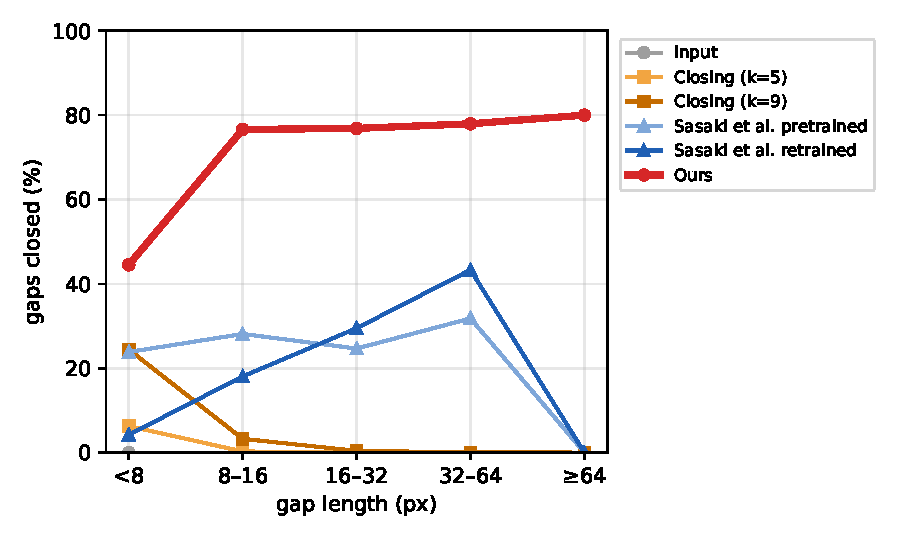
\includegraphics[width=0.75\textwidth]{figures/fig_gap_closure_by_length_all.pdf}
  \caption{Fraction of erased segments closed as a function of segment length. The
  last bin ($\geq$64 pixels) contains only 15 segments.}
  \label{fig:gap_length}
\end{figure}

\paragraph{Qualitative results.} Figure~\ref{fig:qualitative} shows crops centered on
the largest erased segment of the four test images selected for visualization. Our model
reconstructs long missing stretches of straight and curved strokes with the correct
thickness, continues strokes through junctions, and leaves the rest of the drawing
untouched; the few errors (red and blue in its error maps) are mostly one-pixel
deviations along the boundary of the completed strokes. The pretrained Sasaki et al.\
network closes several of the gaps but alters the drawing elsewhere, for example by
adding spurious strokes in the first row. The retrained network produces strokes of
the right thickness, but it leaves part of the long gap of the first row open, and
its error maps show small deviations along nearly all existing strokes, where our
model reproduces the input exactly.

\begin{figure}[t]
  \centering
  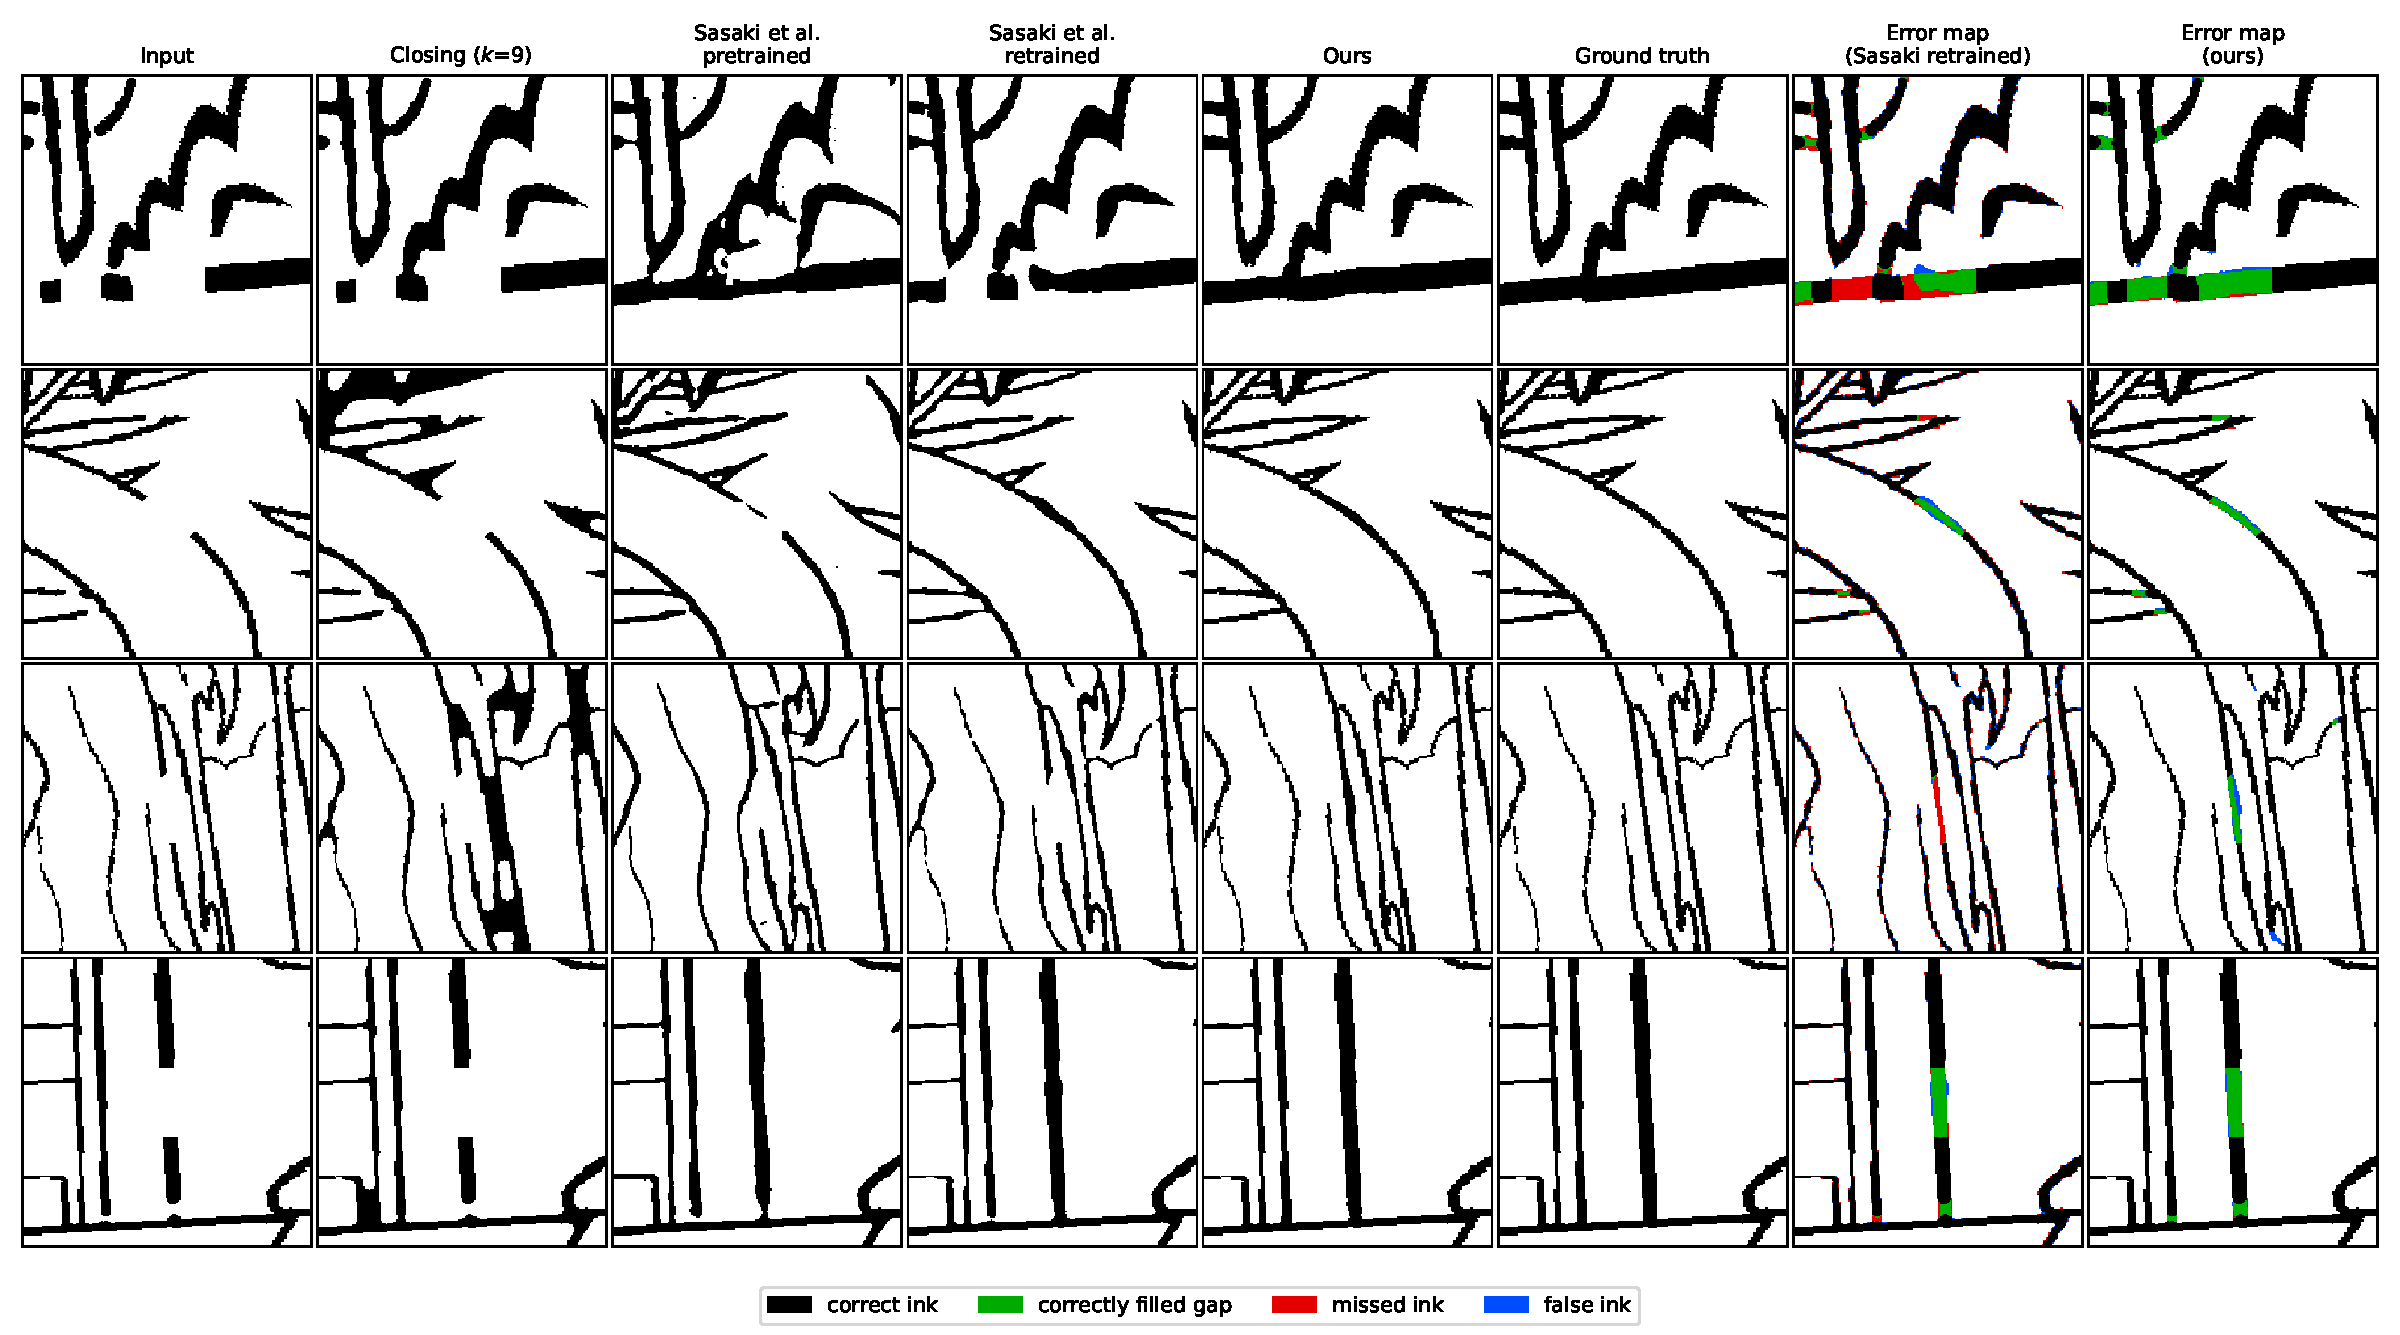
\includegraphics[width=\textwidth]{figures/fig_qualitative_zoom_all.pdf}
  \caption{Qualitative results on the four visualization test images, cropped to a
  $224\times 224$ window centered on the largest erased segment. Columns: corrupted
  input, morphological closing ($k=9$), the pretrained and retrained Sasaki et al.\
  networks, our binarized output, ground truth, and the error maps of the retrained
  Sasaki et al.\ network and of our model (black: correct ink; green: erased ink
  correctly redrawn; red: missed ink; blue: false ink).}
  \label{fig:qualitative}
\end{figure}

\paragraph{Failure cases.} Figure~\ref{fig:failure} shows the three test images with
the lowest fill F1 among those with at least 200 erased pixels. The dominant failure
mode is a long erased stretch of a curved contour whose shape cannot be inferred
from its endpoints alone, as in the lobes of the leaf in the first row: the model
leaves these gaps open instead of guessing a continuation. The retrained Sasaki et
al.\ network also leaves these same gaps open. A second failure mode appears in
regions with several close, nearly parallel strokes or fine hatching (second and
third rows), where the model completes some strokes only partially or adds ink
slightly off the true stroke. Even in these images, the model does not produce the
ink blobs that closing creates.

\begin{figure}[t]
  \centering
  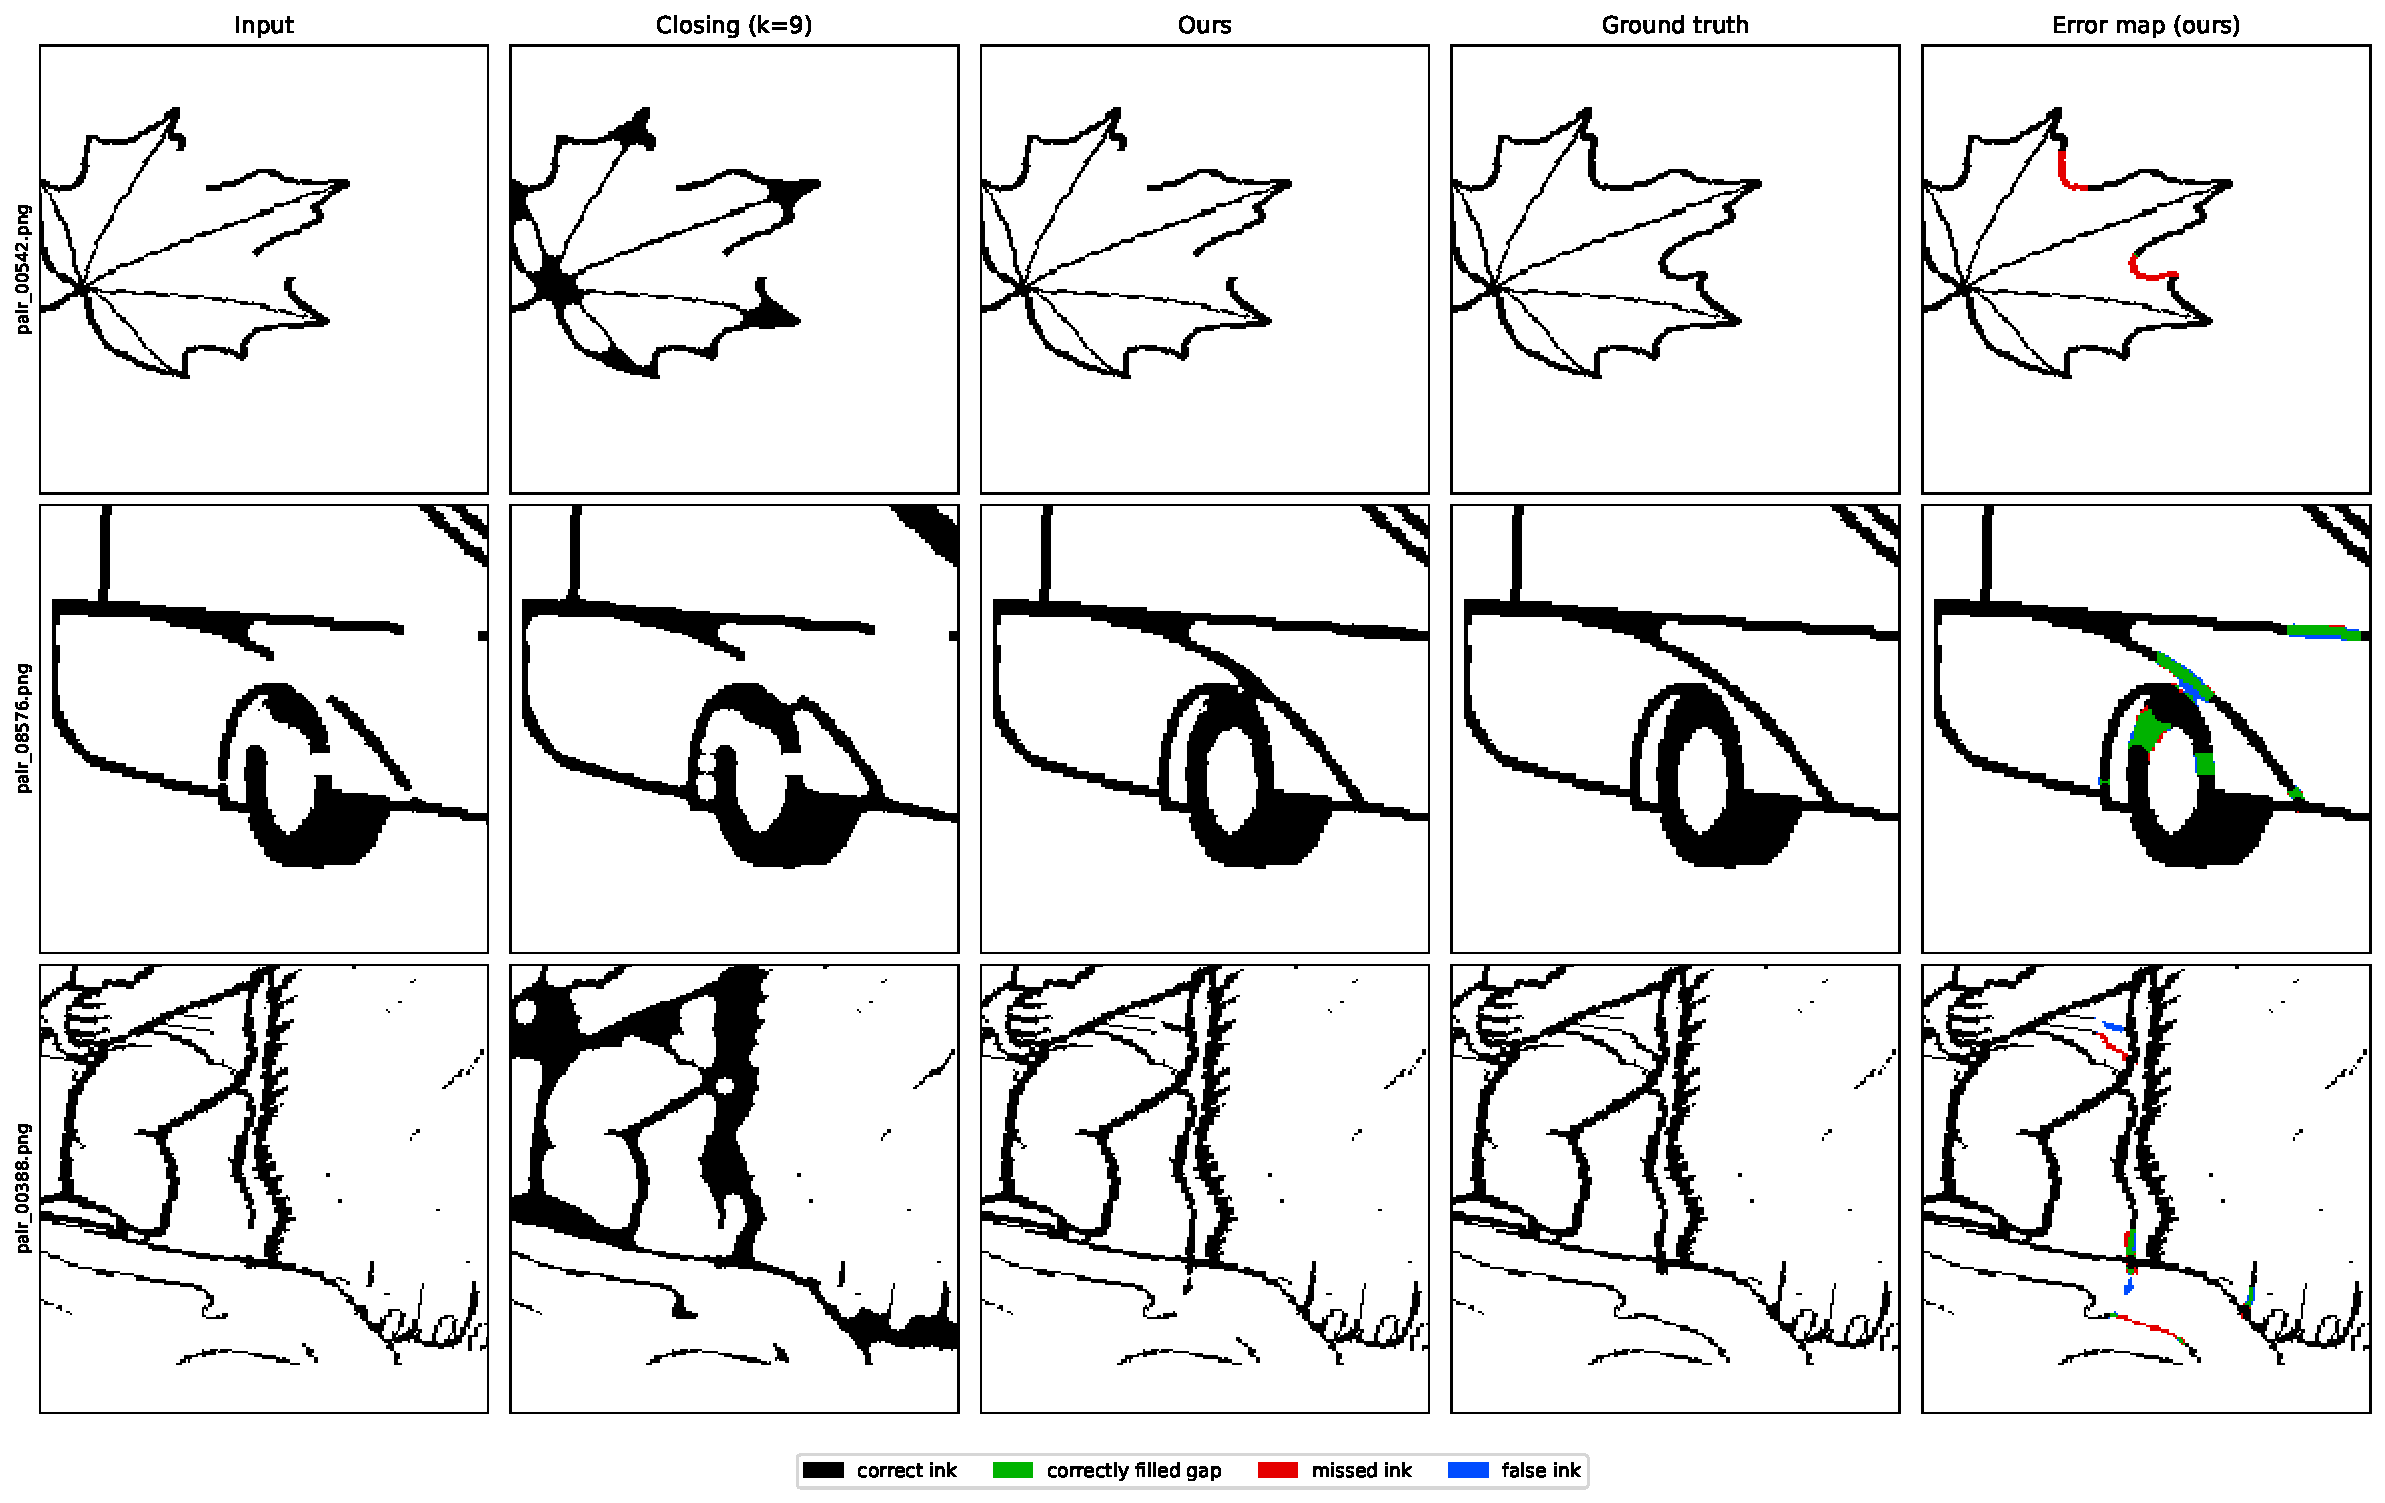
\includegraphics[width=\textwidth]{figures/fig_failure_cases.pdf}
  \caption{Failure cases: the three test images with the lowest fill F1 of our model
  among images with at least 200 erased pixels. Columns: corrupted input,
  morphological closing ($k=9$), our binarized output, ground truth, and the error map
  of our output, with the same color code as Figure~\ref{fig:qualitative}.}
  \label{fig:failure}
\end{figure}

\paragraph{Computational cost.} Our model has 43.4\,M parameters. Inference on one
$896\times 896$ image takes 91.6\,ms in half precision on an NVIDIA Tesla T4 GPU
(forward pass only, excluding loading and binarization), with a peak GPU memory use
of 1.24\,GB, which makes it practical as an interactive preprocessing step before
coloring. The Sasaki et al.\ network is considerably lighter, with 5.5\,M parameters
and a peak memory use of 0.13\,GB; on the same GPU it takes 11.3\,ms per image in
half precision and 23.0\,ms in single precision, in both cases including the transfer
of the image to and from the GPU. Because the timings of the two methods were measured
slightly differently, the comparison is only approximate, but it indicates that our
model is roughly an order of magnitude more expensive, a cost that remains small
compared with that of manual gap repair.

\section{Ablation Study}
\label{sec:ablation}

To assess the contribution of the individual components of InkCloser, we compared
the full model with six variants, evaluated with the protocol of
Section~\ref{sec:metrics} on the same 1\,000 test images. Each variant removes one
component, or several, from the full model:
\begin{itemize}
\item \emph{w/o 28$\times$28 attention}: the six bottleneck transformer blocks are
  removed, and the bottleneck features go directly to the decoder.
\item \emph{w/o 56$\times$56 branch}: the dilated residual stack and the three
  transformer blocks on the $56\times 56$ skip connection are removed.
\item \emph{w/o gated conv}: every gated convolution of the encoder is replaced by a
  standard convolution with the same kernel size, stride, and number of channels.
\item \emph{w/o local (gap) Dice}: the gap Dice term is removed from the loss
  ($\beta_{\mathrm{gap}} = 0$).
\item \emph{Plain U-Net + our loss}: the U-Net alone, with standard convolutions and
  without either context module, trained with the full loss.
\item \emph{Plain U-Net + BCE}: the same network trained with an unweighted binary
  cross-entropy only ($\lambda_h = 1$, $\beta_{\mathrm{dice}} = \beta_{\mathrm{gap}} = 0$).
\end{itemize}
Removed modules are replaced by the identity, so the rest of the network (encoder,
skip connections, decoder, and head) is unchanged. To keep the cost of the study
manageable, the full model and all variants except the first are trained for one
epoch (2\,250 steps) instead of five, with the optimizer, learning rates,
learning-rate schedule, augmentation, and random seed of Section~\ref{sec:method}.
The variant without bottleneck attention is instead compared with the full model at
the training length of the reported model, because one epoch is not enough for this
comparison, as discussed below. The absolute
values in Table~\ref{tab:ablation} are therefore lower than those of the reported
model (Table~\ref{tab:main_results}), and only the differences between variants
trained under the same budget are meaningful; the comparison of interest is
between the full model and each variant trained under the same budget. Differences
are tested with the same paired bootstrap as in Section~\ref{sec:results}, against
the full model trained for one epoch. Table~\ref{tab:ablation} reports all metrics
in percent, except the number of parameters and of leaks per image; each value is
followed by half the width of its 95\% bootstrap confidence interval, and the best
value of each column is in bold.

\begin{table}[t]
\centering
\caption{Ablation study, one epoch per variant.}
\label{tab:ablation}
\small
\resizebox{\linewidth}{!}{%
\begin{tabular}{lccccccc}
\toprule
Variant & \shortstack{Params\\(M)} & \shortstack{Fill F1\\($\tau$=0) $\uparrow$} & \shortstack{Fill F1\\($\tau$=2) $\uparrow$} & \shortstack{Gap\\closure $\uparrow$} & \shortstack{Bucket\\acc. $\uparrow$} & \shortstack{Leaks /\\image $\downarrow$} & \shortstack{Leak-free\\images $\uparrow$} \\
\midrule
InkCloser (full) & 43.4 & \textbf{76.6}{\scriptsize$\pm$0.7} & 91.5{\scriptsize$\pm$0.5} & \textbf{42.2}{\scriptsize$\pm$1.0} & 90.0{\scriptsize$\pm$0.7} & 3.49{\scriptsize$\pm$0.30} & \textbf{26.9}{\scriptsize$\pm$2.8} \\
w/o 56$\times$56 branch & 35.1 & 76.3{\scriptsize$\pm$0.7} & \textbf{91.8}{\scriptsize$\pm$0.5} & 38.8{\scriptsize$\pm$0.9} & \textbf{90.5}{\scriptsize$\pm$0.6} & \textbf{3.31}{\scriptsize$\pm$0.28} & 26.4{\scriptsize$\pm$2.7} \\
w/o gated conv & 37.4 & 69.5{\scriptsize$\pm$0.8} & 86.3{\scriptsize$\pm$0.6} & 41.2{\scriptsize$\pm$1.0} & 87.5{\scriptsize$\pm$0.8} & 4.26{\scriptsize$\pm$0.36} & 21.2{\scriptsize$\pm$2.5} \\
w/o local (gap) Dice & 43.4 & 71.6{\scriptsize$\pm$0.9} & 87.4{\scriptsize$\pm$0.7} & 31.0{\scriptsize$\pm$1.0} & 85.0{\scriptsize$\pm$0.9} & 5.60{\scriptsize$\pm$0.44} & 14.7{\scriptsize$\pm$2.2} \\
Plain U-Net + our loss & 10.2 & 67.9{\scriptsize$\pm$0.8} & 85.9{\scriptsize$\pm$0.6} & 27.3{\scriptsize$\pm$0.8} & 84.8{\scriptsize$\pm$0.9} & 5.52{\scriptsize$\pm$0.42} & 11.5{\scriptsize$\pm$1.9} \\
Plain U-Net + BCE & 10.2 & 66.1{\scriptsize$\pm$0.9} & 85.5{\scriptsize$\pm$0.7} & 18.6{\scriptsize$\pm$0.9} & 77.8{\scriptsize$\pm$1.2} & 8.71{\scriptsize$\pm$0.76} & 10.4{\scriptsize$\pm$1.8} \\
\bottomrule
\end{tabular}}
\end{table}

\paragraph{Loss function.} The gap Dice term is the component whose removal has the
largest effect. Without it, gap closure drops from 42.2\% to 31.0\% (11.2 percentage
points, 95\% CI [10.6, 11.8]), bucket accuracy from 90.0\% to 85.0\%, and the share of
leak-free images from 26.9\% to 14.7\%, while the number of leaks per image rises from
3.49 to 5.60. Its fill F1 also decreases by 5.0 points. This is consistent with the
motivation of the term: the global loss terms are dominated by the intact parts of
the drawing, and the gap Dice term adds a training signal that is specific to the
completed regions. The loss also matters without the context modules: on the plain
U-Net, replacing the unweighted cross-entropy with our loss raises gap closure from
18.6\% to 27.3\% and bucket accuracy from 77.8\% to 84.8\%, and lowers the number of
leaks per image from 8.71 to 5.52.

\paragraph{Gated convolutions.} Replacing the gated convolutions with standard ones
reduces fill F1 by 7.1 points at $\tau=0$ (from 76.6\% to 69.5\%) and by 5.2 points at
$\tau=2$, bucket accuracy by 2.5 points, and the share of leak-free images by 5.7
points (paired bootstrap $p \le 0.001$ for fill F1 at $\tau=0$, bucket accuracy, and
leak-free images). Gap closure decreases less, by 1.0 point (95\% CI [0.4, 1.7]). The variant without gates thus closes almost as many gaps, but the ink it
adds is less accurate. We attribute this to the role of the gates in separating
reliable input from the gaps, which lets the network copy intact strokes and place new
ink more precisely; this interpretation is consistent with, but not proven by, these
results.

\paragraph{Context modules.} Removing the $56\times 56$ branch reduces gap closure by
3.4 points (95\% CI [2.8, 4.0]), while its other metrics stay close to those of the
full model, which suggests that the branch mainly helps the network complete gaps
rather than reproduce the rest of the drawing. The $28\times 28$ bottleneck attention
is not included in Table~\ref{tab:ablation}. Its six transformer blocks account for
almost half of the parameters of the model (19\,M of 43.4\,M), and one epoch is not
enough to assess them: at that budget, the variant without them obtained a higher
bucket accuracy and more leak-free images than the full model, and both differences
reversed or disappeared when the two models were trained for longer. We therefore
compare these two configurations at the training length of the reported model, at the
end of this section.

\paragraph{Architecture as a whole.} Taken together, the components of InkCloser
improve every metric of the plain U-Net trained with the same loss: gap closure rises
from 27.3\% to 42.2\%, fill F1 from 67.9\% to 76.6\%, bucket accuracy from 84.8\% to
90.0\%, and the share of leak-free images from 11.5\% to 26.9\% ($p \le 0.001$ for all
four). Relative to the plain U-Net trained with cross-entropy, the combination of our
architecture and loss more than doubles gap closure (from 18.6\% to 42.2\%) under the
same budget. The reported model, trained five times longer, reaches a much higher gap
closure (70.5\%) than the full model trained for one epoch (42.2\%), while its fill F1
at $\tau=2$ differs by only 1.3 points; this suggests that the structural metrics
benefit most from longer training, and that the ranking of the variants could change
under the full schedule, in particular for components whose effect at one epoch is
small.

\begin{table}[t]
\centering
\caption{Bottleneck attention at the training length of the reported model.}
\label{tab:ablation_long}
\small
\resizebox{\linewidth}{!}{%
\begin{tabular}{lccccccc}
\toprule
Variant & \shortstack{Params\\(M)} & \shortstack{Fill F1\\($\tau$=0) $\uparrow$} & \shortstack{Fill F1\\($\tau$=2) $\uparrow$} & \shortstack{Gap\\closure $\uparrow$} & \shortstack{Bucket\\acc. $\uparrow$} & \shortstack{Leaks /\\image $\downarrow$} & \shortstack{Leak-free\\images $\uparrow$} \\
\midrule
InkCloser (full) & 43.4 & \textbf{80.9}{\scriptsize$\pm$0.6} & \textbf{94.1}{\scriptsize$\pm$0.4} & 59.1{\scriptsize$\pm$1.2} & \textbf{94.2}{\scriptsize$\pm$0.4} & \textbf{1.81}{\scriptsize$\pm$0.18} & \textbf{42.4}{\scriptsize$\pm$3.0} \\
w/o 28$\times$28 attention & 24.4 & 80.2{\scriptsize$\pm$0.6} & 93.7{\scriptsize$\pm$0.4} & \textbf{62.6}{\scriptsize$\pm$1.0} & 94.0{\scriptsize$\pm$0.4} & 1.88{\scriptsize$\pm$0.18} & 41.2{\scriptsize$\pm$2.9} \\
\bottomrule
\end{tabular}}
\end{table}

\paragraph{Bottleneck attention.} Table~\ref{tab:ablation_long} compares the full
model and the variant without bottleneck attention, both retrained for the training
length of the reported model with the settings and random seed of the one-epoch study
and evaluated on the same 1\,000 test images (same format as
Table~\ref{tab:ablation}). The full model is better in fill F1 at $\tau=0$ (+0.7
points, 95\% CI [0.4, 1.0]) and, by a small margin, in bucket accuracy (+0.2 points,
95\% CI [0.04, 0.4]), and the two models do not differ significantly in leak-free
images (+1.2 points, 95\% CI [$-0.8$, 3.2]). The variant without bottleneck attention,
however, closes more gaps (+3.6 points, 95\% CI [3.1, 4.2]), as it already did at one
epoch; it closes more gaps in every length bin from 8 to 64 pixels, with the largest
difference (7.5 points) for gaps between 32 and 64 pixels. In our runs, the bottleneck
attention thus slightly improves the precision of the added ink but does not help the
model close gaps, while it accounts for 19\,M of the 43.4\,M parameters. Both retrained models also close fewer gaps than the reported model
(59.1\% and 62.6\%, against 70.5\% in Table~\ref{tab:main_results}), although the retrained full model has a higher
fill F1 (80.9\% against 78.5\%). The retrained full model and the reported model have
the same architecture, loss, and training length and come from different training
runs, which suggests that gap closure varies considerably from one run to another. We
have not measured this variance, which would require several training runs per
configuration, and the difference between the two configurations should be read with
this in mind.

\section{Discussion and Future Work}
\label{sec:discussion}

The results show that the mask-free formulation is learnable with the proposed
architecture and loss, and that the resulting model turns drawings in which a third
of the regions cannot be filled correctly into drawings in which 94.7\% of them can.
The comparison with \citet{sasaki2017joint} also shows that closing gaps visually is
not sufficient for this application: a method that regenerates the whole drawing can
recover a large part of the missing ink and still produce more leaks than the
unrestored input, because any stroke it weakens elsewhere becomes a new gap.
Preserving the input exactly outside the gaps is as important as filling them.
Several points limit the current conclusions and set the direction for further work.

\paragraph{Remaining leaks.} Although the model separates 94.0\% of the merged
regions, a single remaining gap is enough to spoil a bucket fill, and 55.0\% of the
restored images still contain at least one leak; region count accuracy (38.0\%)
reflects the same effect. From the point of view of a user, however, the remaining
work is reduced from about 15 corrections per image to one or two in most cases.
Weighting the loss towards gaps that actually merge regions, rather than towards all
hole pixels equally, and improving the closure of very short gaps are two direct ways
to increase the fraction of leak-free drawings.

\paragraph{Baselines.} The retrained Sasaki et al.\ network follows the
original training recipe, so its difference from our model combines the effects of
architecture, loss, and optimizer. Training the same architecture with our loss would
separate the contribution of the architecture from that of the loss.
Other comparisons are also left for future work: gap-tolerant region segmentation
such as trapped-ball filling \citep{zhang2009vectorizing}, endpoint-extension heuristics \citep{fourey2018flat}, and mask-guided inpainting methods run with an oracle hole mask as an
upper-bound reference.

\paragraph{Synthetic corruption.} All numbers are obtained with synthetic corruption
applied to already-clean line art (Section~\ref{sec:dataset}). This lets us construct
paired data at scale and compute exact hole masks for training and evaluation, but it
leaves open the question of how well the restoration transfers to gaps produced by
real production processes, such as scanning noise, lossy compression, or line
thinning, which may differ in shape and scale from the synthetic corruption. The
modest zero-shot results of the pretrained Sasaki et al.\ network on our data
illustrate how strongly learned gap-closing models can depend on their training
distribution. Validating the approach on real, naturally occurring gaps is planned
future work.

\paragraph{Metrics.} Region count accuracy is sensitive to any single remaining
error in an image, which makes it a conservative metric, and the bucket and leak
metrics treat all regions equally regardless of their size. A metric that reflects
the practical cost of a remaining gap more closely, for example by weighting leaks by
the area of the regions they affect, may be more informative for this application.

\paragraph{Scope.} The current model operates on a single fixed resolution
($896\times 896$) and on the line style of coloring pages. Generalization to other
resolutions, line styles, and stroke widths has not been evaluated.

\section{Conclusion}

We formulated the restoration of broken lines in line art, for the purpose
of enabling flood-fill coloring, as a mask-free task in which the network must
locate and close gaps without access to a hole mask at inference time. We
described a network combining gated convolutions, a dilated context stack, and
two-scale self-attention, a loss that combines hole-weighted cross-entropy with
global and gap-local Dice terms, and evaluation metrics centered on gap closure and
simulated paint-bucket behavior rather than on pixel accuracy. On a held-out test set
of 1\,000 images, the model closes 70.5\% of the erased segments, with a closure rate
that stays above 76\% for gaps from 8 to more than 64 pixels long, raises the
fraction of correctly paintable regions from 64.1\% to 94.7\%, reduces leaks by
90.5\%, and makes 45.0\% of the drawings entirely leak-free, while preserving the ink
already present in the input. Neither morphological closing nor the joint gap
detection and inpainting network of \citet{sasaki2017joint}, even when retrained on
the same data, closes more than 26.6\% of the gaps or improves on the bucket accuracy
of the unrestored input. Comparing against further baselines and evaluating on naturally occurring rather than synthetic gaps
are the next steps of this work.

\section*{Funding}
This work has been financed by Project PID2024-160996OB-I00, under grant agreement
MICIU/AEI/10.13039/501100011033 and FEDER, UE, and by Generalitat de Catalunya (AGAUR)
under grant agreement 2021-SGR-00478.

\section*{Code and Data Availability}
The source code for dataset generation, model training and evaluation and the pretrained model weights are
available at \url{https://github.com/rtous/inkcloser} \citep{codeInkCloser}.
The InkCloser Dataset of 55\,000 corrupted and clean line-art pairs is publicly available \citep{datasetInkCloser}.

\bibliographystyle{plainnat}
\bibliography{references} 

\end{document}
